% Copyright 2020 by Till Tantau
%
% This file may be distributed and/or modified
%
% 1. under the LaTeX Project Public License and/or
% 2. under the GNU Free Documentation License.
%
% See the file doc/generic/pgf/licenses/LICENSE for more details.
\columnratio{0.55}
\begin{paracol}{2}
\section{Tutorial: A Petri-Net for Hagen}
\switchcolumn
\section{教程:用于Hagen的Petri网}
\switchcolumn[0]*%%%%%%%%%%%%
In this second tutorial we explore the node mechanism of \tikzname\ and
\pgfname.
\switchcolumn
在这个第二个教程中,我们将探索\tikzname\ 和 \pgfname\ 的节点机制。

\switchcolumn[0]*%%%%%%%%%%%%
Hagen must give a talk tomorrow about his favorite formalism for distributed
systems: Petri nets! Hagen used to give his talks using a blackboard and
everyone seemed to be perfectly content with this. Unfortunately, his audience
has been spoiled recently with fancy projector-based presentations and there
seems to be a certain amount of peer pressure that his Petri nets should also
be drawn using a graphic program. One of the professors at his institute
recommends \tikzname\ for this and Hagen decides to give it a try.
\switchcolumn
Hagen必须在明天做关于他最喜欢的分布式系统形式主义——Petri网的演讲!Hagen过去通常使用黑板来进行演讲,而且每个人似乎对此都非常满意。不幸的是,最近他的观众被时髦的投影仪演示所宠坏了,似乎有一定的压力要求他的Petri网也必须使用图形程序绘制。他所在学院的一位教授推荐使用\tikzname\ ,于是Hagen决定试一试。

\switchcolumn[0]*%%%%%%%%%%%%
\subsection{Problem Statement}
\switchcolumn
\subsection{问题陈述}
\switchcolumn[0]*%%%%%%%%%%%%
For his talk, Hagen wishes to create a graphic that demonstrates how a net with
place capacities can be simulated by a net without capacities. The graphic
should look like this, ideally:
\switchcolumn
为了他的演讲,Hagen希望创建一个图形,演示带有位置容量的网如何通过没有容量的网进行模拟。理想情况下,图形应该如下所示:
\switchcolumn[0]*%%%%%%%%%%%%
\begin{quote}
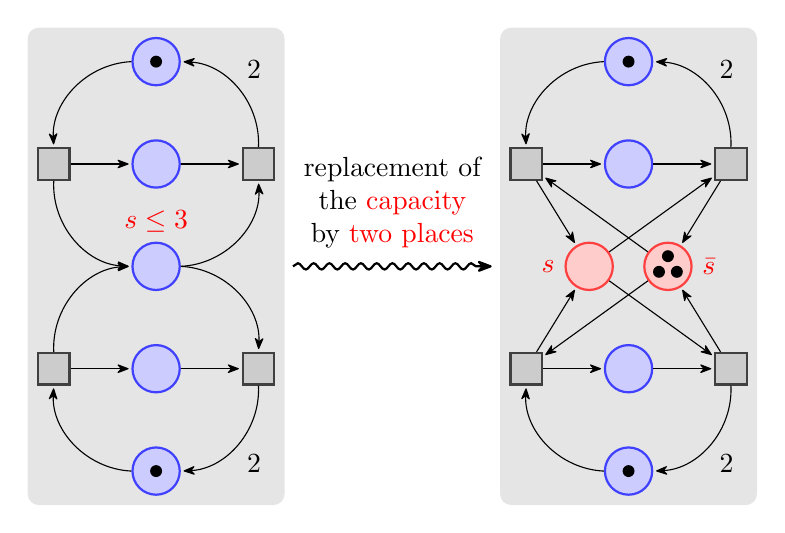
\begin{tikzpicture}
  [node distance=1.3cm,>={Stealth[round]},bend angle=45,auto,
   place/.style={circle,thick,draw=blue!75,fill=blue!20,minimum size=6mm},
   red place/.style={place,draw=red!75,fill=red!20},
   transition/.style={rectangle,thick,draw=black!75,fill=black!20,minimum size=4mm},
   every label/.style={red},on grid]

  \begin{scope}
    % First net
    \node [place,tokens=1] (w1)                                    {};
    \node [place] (c1) [below=of w1]                      {};
    \node [place] (s)  [below=of c1,label=above:$s\le 3$] {};
    \node [place] (c2) [below=of s]                       {};
    \node [place,tokens=1] (w2) [below=of c2]                      {};

    \node [transition] (e1) [left=of c1] {}
      edge [pre,bend left]                  (w1)
      edge [post,bend right]                (s)
      edge [post]                           (c1);

    \node [transition] (e2) [left=of c2] {}
      edge [pre,bend right]                 (w2)
      edge [post,bend left]                 (s)
      edge [post]                           (c2);

    \node [transition] (l1) [right=of c1] {}
      edge [pre]                            (c1)
      edge [pre,bend left]                  (s)
      edge [post,bend right] node[swap] {2} (w1);

    \node [transition] (l2) [right=of c2] {}
      edge [pre]                            (c2)
      edge [pre,bend right]                 (s)
      edge [post,bend left]  node {2}       (w2);
  \end{scope}

  \begin{scope}[xshift=6cm]
    % Second net
    \node [place,tokens=1]
                      (w1')                                                {};
    \node [place]     (c1') [below=of w1']                                 {};
    \node [red place] (s1') [below=of c1',xshift=-5mm,label=left:$s$]      {};
    \node [red place,tokens=3]
                      (s2') [below=of c1',xshift=5mm,label=right:$\bar s$] {};
    \node [place]     (c2') [below=of s1',xshift=5mm]                      {};
    \node [place,tokens=1]
                      (w2') [below=of c2']                                 {};

    \node [transition] (e1') [left=of c1'] {}
      edge [pre,bend left]                  (w1')
      edge [post]                           (s1')
      edge [pre]                            (s2')
      edge [post]                           (c1');

    \node [transition] (e2') [left=of c2'] {}
      edge [pre,bend right]                 (w2')
      edge [post]                           (s1')
      edge [pre]                            (s2')
      edge [post]                           (c2');

    \node [transition] (l1') [right=of c1'] {}
      edge [pre]                            (c1')
      edge [pre]                            (s1')
      edge [post]                           (s2')
      edge [post,bend right] node[swap] {2} (w1');

    \node [transition] (l2') [right=of c2'] {}
      edge [pre]                            (c2')
      edge [pre]                            (s1')
      edge [post]                           (s2')
      edge [post,bend left]  node {2}       (w2');
  \end{scope}

  \begin{scope}[on background layer]
    \node (r1) [fill=black!10,rounded corners,fit=(w1)(w2)(e1)(e2)(l1)(l2)] {};
    \node (r2) [fill=black!10,rounded corners,fit=(w1')(w2')(e1')(e2')(l1')(l2')] {};
  \end{scope}

  \draw [shorten >=1mm,->,thick,decorate,decoration={snake,amplitude=.4mm,segment
      length=2mm,pre=moveto,pre length=1mm,post length=2mm}]
    (r1) -- (r2)
    node [above=1mm,midway,text width=3cm,align=center]
      {replacement of the \textcolor{red}{capacity} by \textcolor{red}{two places}};

\end{tikzpicture}
\end{quote}
\switchcolumn
\begin{quote}
\begin{tikzpicture}
  [node distance=1.3cm,>={Stealth[round]},bend angle=45,auto,%设置了全局的图形属性,包括节点间的距离、箭头样式、曲线角度和自动布局。
   place/.style={circle,thick,draw=blue!75,fill=blue!20,minimum size=6mm},%定义了一个名为place的样式,用于绘制蓝色的圆形节点。
   red place/.style={place,draw=red!75,fill=red!20},%定义了一个名为red place的样式,继承了place样式,并设置节点的颜色为红色。
   transition/.style={rectangle,thick,draw=black!75,fill=black!20,minimum size=4mm},%定义了一个名为transition的样式,用于绘制黑色的矩形节点。
   every label/.style={red},on grid]%设置所有标签的颜色为红色。将图形元素对齐到网格。

  \begin{scope}%定义了一个作用域,在其中绘制了第一张网的节点和变迁。
    % 第一张网 这些代码创建了第一个网格的五个节点,并设置了它们的样式和标签。
    \node [place,tokens=1] (w1)                                    {};%定义了一个带有1个令牌的蓝色节点,并将其命名为w1。
    \node [place] (c1) [below=of w1]                      {c1};
    \node [place] (s)  [below=of c1,label=above:$s\le 3$] {s};
    \node [place] (c2) [below=of s]                       {c2};
    \node [place,tokens=1] (w2) [below=of c2]                      {};

    \node [transition] (e1) [left=of c1] {e1}%%定义了一个黑色的变迁节点,并将其命名为e1,并将其放置在节点c1的左侧。
      %从当前处理的变迁节点出发,画一条向左弯曲且具有先行样式的边,连接到名为 w1 的库所节点。
      edge [pre,bend left]                  (w1)%在变迁e1和节点w1之间绘制了一个向前的弧线,并设置弯曲角度。
      edge [post,bend right]                (s)%在变迁e1和节点s之间绘制了一个向后的弧线,并设置弯曲角度。
      edge [post]                           (c1);

    \node [transition] (e2) [left=of c2] {e2}
      edge [pre,bend right]                 (w2)
      edge [post,bend left]                 (s)
      edge [post]                           (c2);

    \node [transition] (l1) [right=of c1] {l1}
      edge [pre]                            (c1)
      edge [pre,bend left]                  (s)
      edge [post,bend right] node[swap] {2} (w1);

    \node [transition] (l2) [right=of c2] {l2}
      edge [pre]                            (c2)
      edge [pre,bend right]                 (s)
      edge [post,bend left]  node {2}       (w2);
  \end{scope}

  \begin{scope}[xshift=6cm]%定义了一个位移6cm的作用域,在其中绘制了第二张网的节点和变迁。
    % 第二张网
    \node [place,tokens=1]
                      (w1')                                                {};
    \node [place]     (c1') [below=of w1']                                 {};
    \node [red place] (s1') [below=of c1',xshift=-5mm,label=left:$s$]      {};
    \node [red place,tokens=3]
                      (s2') [below=of c1',xshift=5mm,label=right:$\bar s$] {};
    \node [place]     (c2') [below=of s1',xshift=5mm]                      {};
    \node [place,tokens=1]
                      (w2') [below=of c2']                                 {};

    \node [transition] (e1') [left=of c1'] {}
      edge [pre,bend left]                  (w1')
      edge [post]                           (s1')
      edge [pre]                            (s2')
      edge [post]                           (c1');

    \node [transition] (e2') [left=of c2'] {}
      edge [pre,bend right]                 (w2')
      edge [post]                           (s1')
      edge [pre]                            (s2')
      edge [post]                           (c2');

    \node [transition] (l1') [right=of c1'] {}
      edge [pre]                            (c1')
      edge [pre]                            (s1')
      edge [post]                           (s2')
      edge [post,bend right] node[swap] {2} (w1');

    \node [transition] (l2') [right=of c2'] {}
      edge [pre]                            (c2')
      edge [pre]                            (s1')
      edge [post]                           (s2')
      edge [post,bend left]  node {2}       (w2');
  \end{scope}

  \begin{scope}[on background layer]
    \node (r1) [fill=black!10,rounded corners,fit=(w1)(w2)(e1)(e2)(l1)(l2)] {};%定义了一个名称为r1的节点,它是包围节点w1、w2、e1、e2、l1和l2的一个矩形框,并设置其背景色。
    \node (r2) [fill=black!10,rounded corners,fit=(w1')(w2')(e1')(e2')(l1')(l2')] {};
  \end{scope}

  %绘制了一条从节点r1到节点r2的有箭头的线条,并设置了线条的样式。
  \draw [shorten >=1mm,->,thick,decorate,decoration={snake,amplitude=.4mm,segment
      length=2mm,pre=moveto,pre length=1mm,post length=2mm}]
    (r1) -- (r2)
    node [above=1mm,midway,text width=3cm,align=center]
      {用\textcolor{red}{两个位置}替换\textcolor{red}{容量}};%在线条的中点上方添加了一个节点,并设置了节点的样式和文本内容。

\end{tikzpicture}
\end{quote}
\switchcolumn[0]*%%%%%%%%%%%%
\subsection{Setting up the Environment}
\switchcolumn
\subsection{设置环境}
\switchcolumn[0]*%%%%%%%%%%%%
For the picture Hagen will need to load the \tikzname\ package as did Karl in
the previous tutorial. However, Hagen will also need to load some additional
\emph{library packages} that Karl did not need. These library packages contain
additional definitions like extra arrow tips that are typically not needed in a
picture and that need to be loaded explicitly.
\switchcolumn
对于图片,Hagen需要加载\tikzname\ 包,就像Karl在前一个教程中所做的一样。然而,Hagen还需要加载一些Karl不需要的额外\emph{库包}。这些库包包含了额外的定义,如通常不需要在图片中使用的额外箭头样式,需要显式地加载。

\switchcolumn[0]*%%%%%%%%%%%%
Hagen will need to load several libraries: The |arrows.meta| library for the
special arrow tip used in the graphic, the |decorations.pathmorphing| library
for the ``snaking line'' in the middle, the |backgrounds| library for the two
rectangular areas that are behind the two main parts of the picture, the |fit|
library to easily compute the sizes of these rectangles, and the |positioning|
library for placing nodes relative to other nodes.
\switchcolumn
Hagen需要加载几个库:|arrows.meta| 库用于图形中使用的特殊箭头样式,|decorations.pathmorphing| 库用于中间的``蛇形线'',|backgrounds| 库用于两个主要部分后面的两个矩形区域,|fit| 库用于轻松计算这些矩形的尺寸,以及|positioning| 库用于相对于其他节点放置节点。

\switchcolumn[0]*%%%%%%%%%%%%
\subsubsection{Setting up the Environment in \LaTeX}
\switchcolumn
\subsubsection{在\LaTeX 中设置环境}
\switchcolumn[0]*%%%%%%%%%%%%
When using \LaTeX\ use:
\begin{codeexample}[code only]
\documentclass{article} % say

\usepackage{tikz}
\usetikzlibrary{arrows.meta,decorations.pathmorphing,backgrounds,positioning,fit,petri}

\begin{document}
\begin{tikzpicture}
  \draw (0,0) -- (1,1);
\end{tikzpicture}
\end{document}
\end{codeexample}
\switchcolumn
在使用\LaTeX 时,使用以下代码:
\begin{codeexample}[code only]
\documentclass{article} % say

\usepackage{tikz}
\usetikzlibrary{arrows.meta,decorations.pathmorphing,backgrounds,positioning,fit,petri}

\begin{document}
\begin{tikzpicture}
  \draw (0,0) -- (1,1);
\end{tikzpicture}
\end{document}
\end{codeexample}

\switchcolumn[0]*%%%%%%%%%%%%
\subsubsection{Setting up the Environment in Plain \TeX}
\switchcolumn
\subsubsection{在Plain \TeX 中设置环境}
\switchcolumn[0]*%%%%%%%%%%%%
When using plain \TeX\ use:
\begin{codeexample}[code only]
%% Plain TeX file
\input tikz.tex
\usetikzlibrary{arrows.meta,decorations.pathmorphing,backgrounds,positioning,fit,petri}
\baselineskip=12pt
\hsize=6.3truein
\vsize=8.7truein
\tikzpicture
  \draw (0,0) -- (1,1);
\endtikzpicture
\bye
\end{codeexample}
\switchcolumn
在使用Plain \TeX 时,使用以下代码:
\begin{codeexample}[code only]
%% Plain TeX file
\input tikz.tex
\usetikzlibrary{arrows.meta,decorations.pathmorphing,backgrounds,positioning,fit,petri}
\baselineskip=12pt
\hsize=6.3truein
\vsize=8.7truein
\tikzpicture
  \draw (0,0) -- (1,1);
\endtikzpicture
\bye
\end{codeexample}

\switchcolumn[0]*%%%%%%%%%%%%
\subsubsection{Setting up the Environment in Con\TeX t}
\switchcolumn
\subsubsection{在Con\TeX t 中设置环境}
\switchcolumn[0]*%%%%%%%%%%%%
When using Con\TeX t, use:
\begin{codeexample}[code only]
%% ConTeXt file
\usemodule[tikz]
\usetikzlibrary[arrows.meta,decorations.pathmorphing,backgrounds,positioning,fit,petri]

\starttext
  \starttikzpicture
    \draw (0,0) -- (1,1);
  \stoptikzpicture
\stoptext
\end{codeexample}

\switchcolumn
在使用Con\TeX t时,使用以下代码:
\begin{codeexample}[code only]
  %% ConTeXt file
  \usemodule[tikz]
  \usetikzlibrary[arrows.meta,decorations.pathmorphing,backgrounds,positioning,fit,petri]
  
  \starttext
    \starttikzpicture
      \draw (0,0) -- (1,1);
    \stoptikzpicture
  \stoptext
  \end{codeexample}

\switchcolumn[0]*%%%%%%%%%%%%
\subsection{Introduction to Nodes}
\switchcolumn
\subsection{节点简介}
\switchcolumn[0]*%%%%%%%%%%%%
In principle, we already know how to create the graphics that Hagen desires
(except perhaps for the snaked line, we will come to that): We start with big
light gray rectangle and then add lots of circles and small rectangle, plus
some arrows.
\switchcolumn
原则上,我们已经知道如何创建Hagen所需的图形(也许除了蛇形线,我们将在后面讨论它):我们从一个大的浅灰色矩形开始,然后添加许多圆圈和小矩形,以及一些箭头。

\switchcolumn[0]*%%%%%%%%%%%%
However, this approach has numerous disadvantages: First, it is hard to change
anything at a later stage. For example, if we decide to add more places to the
Petri nets (the circles are called places in Petri net theory), all of the
coordinates change and we need to recalculate everything. Second, it is hard to
read the code for the Petri net as it is just a long and complicated list of
coordinates and drawing commands -- the underlying structure of the Petri net
is lost.
\switchcolumn
然而,这种方法有许多缺点:首先,在后期更改任何内容都很困难。例如,如果我们决定向Petri网中添加更多的库所(在Petri网理论中,圆圈被称为库所),所有的坐标都会改变,我们需要重新计算所有内容。其次,很难阅读Petri网的代码,因为它只是一个冗长而复杂的坐标和绘图命令列表——Petri网的底层结构丢失了。

\switchcolumn[0]*%%%%%%%%%%%%
Fortunately, \tikzname\ offers a powerful mechanism for avoiding the above
problems: nodes. We already came across nodes in the previous tutorial, where
we used them to add labels to Karl's graphic. In the present tutorial we will
see that nodes are much more powerful.
\switchcolumn
幸运的是,\tikzname\ 提供了一个强大的机制来避免上述问题:节点。在前一个教程中,我们已经了解到节点,我们用它们来为Karl的图形添加标签。在本教程中,我们将看到节点更加强大。

\switchcolumn[0]*%%%%%%%%%%%%
A node is a small part of a picture. When a node is created, you provide a
position where the node should be drawn and a \emph{shape}. A node of shape
|circle| will be drawn as a circle, a node of shape |rectangle| as a rectangle,
and so on. A node may also contain some text, which is why Karl used nodes to
show text. Finally, a node can get a \emph{name} for later reference.
\switchcolumn
节点是图片的一个小部分。当创建一个节点时,需要提供节点应该绘制的位置和一个\emph{形状}。形状为|circle|的节点将绘制为圆,形状为|rectangle|的节点将绘制为矩形,等等。节点还可以包含一些文本,这就是为什么Karl使用节点来显示文本。最后,节点可以获得一个\emph{名称}以供以后引用。

\switchcolumn[0]*%%%%%%%%%%%%
In Hagen's picture we will use nodes for the places and for the transitions of
the Petri net (the places are the circles, the transitions are the rectangles).
Let us start with the upper half of the left Petri net. In this upper half we
have three places and two transitions. Instead of drawing three circles and two
rectangles, we use three nodes of shape |circle| and two nodes of shape
|rectangle|.
\switchcolumn
在Hagen的图片中,我们将使用节点来表示Petri网的库所和变迁(places是圆圈,transitions是矩形)。让我们从左侧Petri网的上半部分开始。在这个上半部分,我们有三个places和两个transitions。我们不使用三个圆圈和两个矩形来绘制,而是使用三个形状为|circle|的节点和两个形状为|rectangle|的节点。%
\switchcolumn[0]*%%%%%%%%%%%%
\begin{dispExample*}{sidebyside}
\begin{tikzpicture}
  \path ( 0,2) node [shape=circle,draw] {}
        ( 0,1) node [shape=circle,draw] {}
        ( 0,0) node [shape=circle,draw] {}
        ( 1,1) node [shape=rectangle,draw] {}
        (-1,1) node [shape=rectangle,draw] {};
\end{tikzpicture}
\end{dispExample*}
\switchcolumn
\begin{dispExample*}{sidebyside}
\begin{tikzpicture}
  \path ( 0,2) node [shape=circle,draw] {}
        ( 0,1) node [shape=circle,draw] {}
        ( 0,0) node [shape=circle,draw] {}
        ( 1,1) node [shape=rectangle,draw] {}
        (-1,1) node [shape=rectangle,draw] {};
\end{tikzpicture}
\end{dispExample*}

\switchcolumn[0]*%%%%%%%%%%%%
Hagen notes that this does not quite look like the final picture, but it seems
like a good first step.
\switchcolumn
Hagen指出,这看起来还不像最终的图片,但它似乎是一个不错的第一步。

\switchcolumn[0]*%%%%%%%%%%%%
Let us have a more detailed look at the code. The whole picture consists of a
single path. Ignoring the |node| operations, there is not much going on in this
path: It is just a sequence of coordinates with nothing ``happening'' between
them. Indeed, even if something were to happen like a line-to or a curve-to,
the |\path| command would not ``do'' anything with the resulting path. So, all
the magic must be in the |node| commands.
\switchcolumn
让我们详细看一下代码。整个图片由一个路径组成。忽略|node|操作,这个路径中没有太多的东西:它只是一系列的坐标,它们之间没有发生任何事情。事实上,即使有什么事情发生,比如画线或曲线,|\path|命令也不会对生成的路径做任何操作。因此,所有的奇迹必须在|node|命令中。

\switchcolumn[0]*%%%%%%%%%%%%
In the previous tutorial we learned that a |node| will add a piece of text at
the last coordinate. Thus, each of the five nodes is added at a different
position. In the above code, this text is empty (because of the empty |{}|).
So, why do we see anything at all? The answer is the |draw| option for the
|node| operation: It causes the ``shape around the text'' to be drawn.
\switchcolumn
在上一篇教程中,我们学到了|node|会在最后一个坐标上添加一段文本。因此,五个节点中的每一个都会添加在不同的位置。在上面的代码中,这段文本是空的(因为是空的|{}|)。那么为什么我们看到了任何东西呢?答案是|node|操作中的|draw|选项:它导致``文本周围的形状''被绘制出来。

\switchcolumn[0]*%%%%%%%%%%%%
So, the code |(0,2) node [shape=circle,draw] {}| means the following: ``In the
main path, add a move-to to the coordinate |(0,2)|. Then, temporarily suspend
the construction of the main path while the node is built. This node will be a
|circle| around an empty text. This circle is to be |draw|n, but not filled or
otherwise used. Once this whole node is constructed, it is saved until after
the main path is finished. Then, it is drawn.'' The following
|(0,1) node [shape=circle,draw] {}| then has the following effect: ``Continue
the main path with a move-to to |(0,1)|. Then construct a node at this position
also. This node is also shown after the main path is finished.'' And so on.
\switchcolumn
所以,代码|(0,2) node [shape=circle,draw] {}|的意思是:在主路径中,添加一个移动到坐标|(0,2)|的操作。然后,在构建主路径时,临时暂停,直到节点被构建完成。这个节点将是一个围绕着空文本的|circle|。这个圆要被绘制,但不填充或以其他方式使用。一旦整个节点构建完成,它就会被保存,直到主路径完成后再被绘制。''接下来的|(0,1) node [shape=circle,draw] {}|的效果是:用一个移动到|(0,1)|的操作继续主路径。然后在这个位置上构建一个节点。这个节点也会在主路径完成后显示。''依此类推。

\switchcolumn[0]*%%%%%%%%%%%%
\subsection{Placing Nodes Using the At Syntax}
\switchcolumn
\subsection{使用At语法放置节点}
\switchcolumn[0]*%%%%%%%%%%%%
Hagen now understands how the |node| operation adds nodes to the path, but it
seems a bit silly to create a path using the |\path| operation, consisting of
numerous superfluous move-to operations, only to place nodes. He is pleased to
learn that there are ways to add nodes in a more sensible manner.
\switchcolumn
Hagen现在明白了|node|操作是如何将节点添加到路径中的,但是只使用|\path|操作创建一个包含许多多余的移动操作的路径来放置节点似乎有点愚蠢。他很高兴地得知有更合理的方法来添加节点。

\switchcolumn[0]*%%%%%%%%%%%%
First, the |node| operation allows one to add |at (|\meta{coordinate}|)| in
order to directly specify where the node should be placed, sidestepping the
rule that nodes are placed on the last coordinate. Hagen can then write the
following:
\switchcolumn
首先,|node|操作允许在|at (|\meta{coordinate}|)|中直接指定节点应该放置的位置,绕过了节点放置在最后一个坐标上的规则。Hagen可以这样写:
%
\begin{dispExample*}{sidebyside}
\begin{tikzpicture}
  \path node at ( 0,2) [shape=circle,draw] {}
        node at ( 0,1) [shape=circle,draw] {}
        node at ( 0,0) [shape=circle,draw] {}
        node at ( 1,1) [shape=rectangle,draw] {}
        node at (-1,1) [shape=rectangle,draw] {};
\end{tikzpicture}
\end{dispExample*}
\switchcolumn
\begin{dispExample*}{sidebyside}
\begin{tikzpicture}
  \path node at ( 0,2) [shape=circle,draw] {}
        node at ( 0,1) [shape=circle,draw] {}
        node at ( 0,0) [shape=circle,draw] {}
        node at ( 1,1) [shape=rectangle,draw] {}
        node at (-1,1) [shape=rectangle,draw] {};
\end{tikzpicture}
\end{dispExample*}

\switchcolumn[0]*%%%%%%%%%%%%
Now Hagen is still left with a single empty path, but at least the path no
longer contains strange move-to's. It turns out that this can be improved
further: The |\node| command is an abbreviation for |\path node|, which allows
Hagen to write:
\switchcolumn
现在Hagen还是得到了一个空路径,但至少路径不再包含奇怪的移动操作了。事实证明,这还可以进一步改进:|\node|命令是|\path node|的缩写形式,这使得Hagen可以这样写:
\switchcolumn[0]*%%%%%%%%%%%
\begin{dispExample*}{sidebyside}
\begin{tikzpicture}
  \node at ( 0,2) [circle,draw] {};
  \node at ( 0,1) [circle,draw] {};
  \node at ( 0,0) [circle,draw] {};
  \node at ( 1,1) [rectangle,draw] {};
  \node at (-1,1) [rectangle,draw] {};
\end{tikzpicture}
\end{dispExample*}
\switchcolumn
\begin{dispExample*}{sidebyside}
\begin{tikzpicture}
  \node at ( 0,2) [circle,draw] {};
  \node at ( 0,1) [circle,draw] {};
  \node at ( 0,0) [circle,draw] {};
  \node at ( 1,1) [rectangle,draw] {};
  \node at (-1,1) [rectangle,draw] {};
\end{tikzpicture}
\end{dispExample*}

\switchcolumn[0]*%%%%%%%%%%%%
Hagen likes this syntax much better than the previous one. Note that Hagen has
also omitted the |shape=| since, like |color=|, \tikzname\ allows you to omit
the |shape=| if there is no confusion.
\switchcolumn
Hagen非常喜欢这种语法,比起之前的语法要好得多。请注意,Hagen还省略了|shape=|,因为像|color=|一样,如果没有混淆,\tikzname 允许省略|shape=|。

\switchcolumn[0]*%%%%%%%%%%%%
\switchcolumn[0]*%%%%%%%%%%%%
\subsection{Using Styles}
\switchcolumn
\subsection{使用样式}
\switchcolumn[0]*%%%%%%%%%%%%
Feeling adventurous, Hagen tries to make the nodes look nicer. In the final
picture, the circles and rectangle should be filled with different colors,
resulting in the following code:
\switchcolumn
Hagen感到充满冒险精神,试图让节点看起来更漂亮。在最终的图片中,圆圈和矩形应该用不同的颜色填充,代码如下所示:
\switchcolumn[0]*%%%%%%%%%%%%
\begin{dispExample*}{sidebyside}
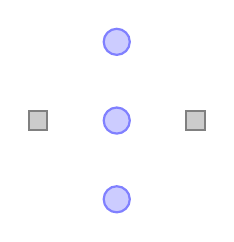
\begin{tikzpicture}[thick]
  \node at ( 0,2) [circle,draw=blue!50,fill=blue!20] {};
  \node at ( 0,1) [circle,draw=blue!50,fill=blue!20] {};
  \node at ( 0,0) [circle,draw=blue!50,fill=blue!20] {};
  \node at ( 1,1) [rectangle,draw=black!50,fill=black!20] {};
  \node at (-1,1) [rectangle,draw=black!50,fill=black!20] {};
\end{tikzpicture}
\end{dispExample*}
\switchcolumn
\begin{dispExample*}{sidebyside,lefthand ratio=0.7}
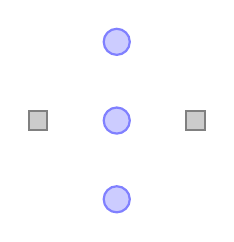
\begin{tikzpicture}[thick]
  \node at ( 0,2) [circle,draw=blue!50,fill=blue!20] {};
  \node at ( 0,1) [circle,draw=blue!50,fill=blue!20] {};
  \node at ( 0,0) [circle,draw=blue!50,fill=blue!20] {};
  \node at ( 1,1) [rectangle,draw=black!50,fill=black!20] {};
  \node at (-1,1) [rectangle,draw=black!50,fill=black!20] {};
\end{tikzpicture}
\end{dispExample*}
\switchcolumn[0]*%%%%%%%%%%%%
While this looks nicer in the picture, the code starts to get a bit ugly.
Ideally, we would like our code to transport the message ``there are three
places and two transitions'' and not so much which filling colors should be
used.
\switchcolumn
虽然这在图片中看起来更漂亮,但代码变得有点丑陋。理想情况下,我们希望我们的代码传达的是"有三个位置和两个转换"这一信息,而不是使用哪些填充颜色。

\switchcolumn[0]*%%%%%%%%%%%%
To solve this problem, Hagen uses styles. He defines a style for places and
another style for transitions:
\switchcolumn
为了解决这个问题,Hagen使用样式。他为位置定义了一个样式,为转换定义了另一个样式:
\switchcolumn[0]*%%%%%%%%%%%%
\begin{dispExample*}{sidebyside,lefthand ratio=0.7}
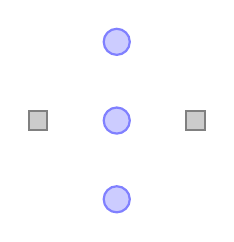
\begin{tikzpicture}
  [place/.style={circle,draw=blue!50,fill=blue!20,thick},
   transition/.style={rectangle,draw=black!50,fill=black!20,thick}]
  \node at ( 0,2) [place] {};
  \node at ( 0,1) [place] {};
  \node at ( 0,0) [place] {};
  \node at ( 1,1) [transition] {};
  \node at (-1,1) [transition] {};
\end{tikzpicture}
\end{dispExample*}
\switchcolumn
\begin{dispExample*}{sidebyside,lefthand ratio=0.7}
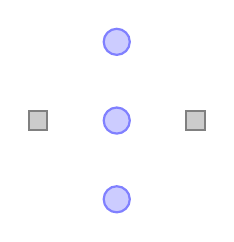
\begin{tikzpicture}
  [place/.style={circle,draw=blue!50,fill=blue!20,thick},
   transition/.style={rectangle,draw=black!50,fill=black!20,thick}]
  \node at ( 0,2) [place] {};
  \node at ( 0,1) [place] {};
  \node at ( 0,0) [place] {};
  \node at ( 1,1) [transition] {};
  \node at (-1,1) [transition] {};
\end{tikzpicture}
\end{dispExample*}


\switchcolumn[0]*%%%%%%%%%%%%
\subsection{Node Size}
\switchcolumn
\subsection{节点大小}
\switchcolumn[0]*%%%%%%%%%%%%
Before Hagen starts naming and connecting the nodes, let us first make sure
that the nodes get their final appearance. They are still too small. Indeed,
Hagen wonders why they have any size at all, after all, the text is empty. The
reason is that \tikzname\ automatically adds some space around the text. The
amount is set using the option |inner sep|. So, to increase the size of the
nodes, Hagen could write:
\switchcolumn
在Hagen开始为节点命名和连接它们之前,我们先确保节点具有最终的外观。它们仍然太小了。实际上,Hagen想知道为什么它们有任何大小,毕竟文本是空的。原因是\tikzname\ 自动在文本周围添加一些空间。这个空间的大小由选项|inner sep|设置。因此,为了增加节点的大小,Hagen可以这样写:
\switchcolumn[0]*%%%%%%%%%%%%
\begin{dispExample*}{sidebyside,lefthand ratio=0.7}
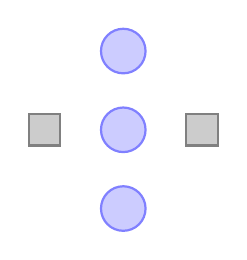
\begin{tikzpicture}
  [inner sep=2mm,
   place/.style={circle,draw=blue!50,fill=blue!20,thick},
   transition/.style={rectangle,draw=black!50,fill=black!20,thick}]
  \node at ( 0,2) [place] {};
  \node at ( 0,1) [place] {};
  \node at ( 0,0) [place] {};
  \node at ( 1,1) [transition] {};
  \node at (-1,1) [transition] {};
\end{tikzpicture}
\end{dispExample*}
\switchcolumn
\begin{dispExample*}{sidebyside,lefthand ratio=0.7}
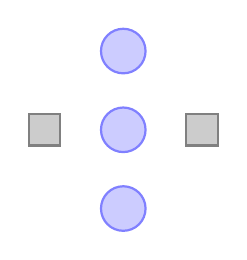
\begin{tikzpicture}
  [inner sep=2mm,
   place/.style={circle,draw=blue!50,fill=blue!20,thick},
   transition/.style={rectangle,draw=black!50,fill=black!20,thick}]
  \node at ( 0,2) [place] {};
  \node at ( 0,1) [place] {};
  \node at ( 0,0) [place] {};
  \node at ( 1,1) [transition] {};
  \node at (-1,1) [transition] {};
\end{tikzpicture}
\end{dispExample*}

\switchcolumn[0]*%%%%%%%%%%%%
However, this is not really the best way to achieve the desired effect. It is
much better to use the |minimum size| option instead. This option allows Hagen
to specify a minimum size that the node should have. If the node actually needs
to be bigger because of a longer text, it will be larger, but if the text is
empty, then the node will have |minimum size|. This option is also useful to
ensure that several nodes containing different amounts of text have the same
size. The options |minimum height| and |minimum width| allow you to specify the
minimum height and width independently.
\switchcolumn
然而,这并不是实现所需效果的最佳方法。更好的方法是使用 |minimum size| 选项。该选项允许 Hagen 指定节点应具有的最小尺寸。如果节点因为较长的文本而需要更大的尺寸,它将变得更大,但如果文本为空,则节点将具有 |minimum size|。该选项还可用于确保包含不同文本量的多个节点具有相同的大小。选项 |minimum height| 和 |minimum width| 允许您单独指定最小高度和宽度。

\switchcolumn[0]*%%%%%%%%%%%%
So, what Hagen needs to do is to provide |minimum size| for the nodes. To be on
the safe side, he also sets |inner sep=0pt|. This ensures that the nodes will
really have size |minimum size| and not, for very small minimum sizes, the
minimal size necessary to encompass the automatically added space.
\switchcolumn
因此,Hagen 需要为节点提供 |minimum size|。为了保险起见,他还设置了 |inner sep=0pt|。这确保节点确实具有 |minimum size|,而不是对于非常小的最小尺寸,仅足以包含自动添加的空间的最小尺寸。
\switchcolumn[0]*%%%%%%%%%%%%
\begin{dispExample*}{sidebyside,lefthand ratio=0.7}
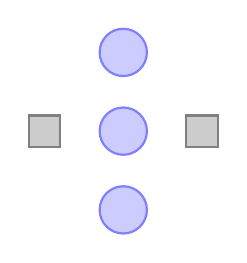
\begin{tikzpicture}
  [place/.style={circle,draw=blue!50,fill=blue!20,thick,
                 inner sep=0pt,minimum size=6mm},
   transition/.style={rectangle,draw=black!50,fill=black!20,thick,
                      inner sep=0pt,minimum size=4mm}]
  \node at ( 0,2) [place] {};
  \node at ( 0,1) [place] {};
  \node at ( 0,0) [place] {};
  \node at ( 1,1) [transition] {};
  \node at (-1,1) [transition] {};
\end{tikzpicture}
\end{dispExample*}
\switchcolumn
\begin{dispExample*}{sidebyside,lefthand ratio=0.7}
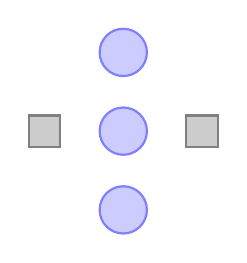
\begin{tikzpicture}
  [place/.style={circle,draw=blue!50,fill=blue!20,thick,
                 inner sep=0pt,minimum size=6mm},
   transition/.style={rectangle,draw=black!50,fill=black!20,thick,
                      inner sep=0pt,minimum size=4mm}]
  \node at ( 0,2) [place] {};
  \node at ( 0,1) [place] {};
  \node at ( 0,0) [place] {};
  \node at ( 1,1) [transition] {};
  \node at (-1,1) [transition] {};
\end{tikzpicture}
\end{dispExample*}


\switchcolumn[0]*%%%%%%%%%%%%
\subsection{Naming Nodes}
\switchcolumn
\subsection{节点命名}
\switchcolumn[0]*%%%%%%%%%%%%
Hagen's next aim is to connect the nodes using arrows. This seems like a tricky
business since the arrows should not start in the middle of the nodes, but
somewhere on the border and Hagen would very much like to avoid computing these
positions by hand.
\switchcolumn
Hagen的下一个目标是使用箭头连接节点。这似乎是一个棘手的问题,因为箭头不应该从节点的中间开始,而应该从边界的某个位置开始。Hagen非常希望避免手动计算这些位置。

\switchcolumn[0]*%%%%%%%%%%%%
Fortunately, \pgfname\ will perform all the necessary calculations for him.
However, he first has to assign names to the nodes so that he can reference
them later on.
\switchcolumn
幸运的是,\pgfname\ 将为他执行所有必要的计算。但是,他首先必须给节点指定名称,以便以后可以引用它们。

\switchcolumn[0]*%%%%%%%%%%%%
There are two ways to name a node. The first is to use the |name=| option. The
second method is to write the desired name in parentheses after the |node|
operation. Hagen thinks that this second method seems strange, but he will soon
change his opinion.
\switchcolumn
有两种方法可以给节点命名。第一种方法是使用 |name=| 选项。第二种方法是在 |node| 操作后的括号中写入所需的名称。Hagen认为第二种方法似乎很奇怪,但他很快会改变自己的看法。
\switchcolumn[0]*%%%%%%%%%%%%
\begin{codeexample}[setup code,hidden]
\tikzset{
    place/.style={circle,draw=blue!50,fill=blue!20,thick,
                  inner sep=0pt,minimum size=6mm},
    transition/.style={rectangle,draw=black!50,fill=black!20,thick,
                       inner sep=0pt,minimum size=4mm}
}
\end{codeexample}
%
\begin{dispExample*}{sidebyside}
% ... set up styles
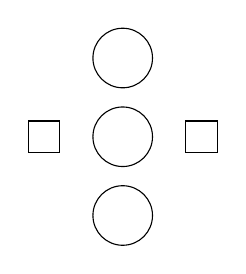
\begin{tikzpicture}
  \node (waiting 1)      at ( 0,2) [place] {};
  \node (critical 1)     at ( 0,1) [place] {};
  \node (semaphore)      at ( 0,0) [place] {};
  \node (leave critical) at ( 1,1) [transition] {};
  \node (enter critical) at (-1,1) [transition] {};
\end{tikzpicture}
\end{dispExample*}
\switchcolumn
\begin{dispExample*}{sidebyside,lefthand ratio=0.7}
% ... set up styles
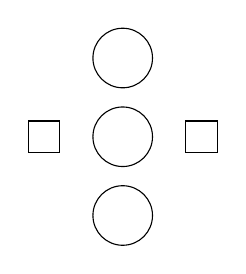
\begin{tikzpicture}
  \node (waiting 1)      at ( 0,2) [place] {};
  \node (critical 1)     at ( 0,1) [place] {};
  \node (semaphore)      at ( 0,0) [place] {};
  \node (leave critical) at ( 1,1) [transition] {};
  \node (enter critical) at (-1,1) [transition] {};
\end{tikzpicture}
\end{dispExample*}

\switchcolumn[0]*%%%%%%%%%%%%
Hagen is pleased to note that the names help in understanding the code. Names
for nodes can be pretty arbitrary, but they should not contain commas, periods,
parentheses, colons, and some other special characters. However, they can
contain underscores and hyphens.
\switchcolumn
Hagen很高兴地注意到,这些名称有助于理解代码。节点的名称可以是任意的,但是不能包含逗号、句点、括号、冒号和其他一些特殊字符。但是,它们可以包含下划线和连字符。

\switchcolumn[0]*%%%%%%%%%%%%
The syntax for the |node| operation is quite liberal with respect to the order
in which node names, the |at| specifier, and the options must come. Indeed, you
can even have multiple option blocks between the |node| and the text in curly
braces, they accumulate. You can rearrange them arbitrarily and perhaps the
following might be preferable:
\switchcolumn
对于 |node| 操作,语法在节点名称、|at| 指定符和选项之间的顺序方面非常自由。实际上,你甚至可以在 |node| 和花括号中的文本之间有多个选项块,它们会累积起来。你可以任意重新排列它们,也许以下代码可能更可取:%
\switchcolumn[0]*%%%%%%%%%%%%
\begin{dispExample*}{sidebyside}
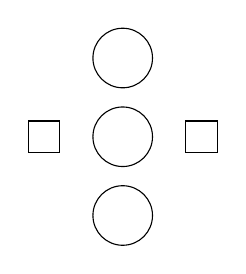
\begin{tikzpicture}
  \node[place]      (waiting 1)      at ( 0,2) {};
  \node[place]      (critical 1)     at ( 0,1) {};
  \node[place]      (semaphore)      at ( 0,0) {};
  \node[transition] (leave critical) at ( 1,1) {};
  \node[transition] (enter critical) at (-1,1) {};
\end{tikzpicture}
\end{dispExample*}
\switchcolumn
\begin{dispExample*}{sidebyside,lefthand ratio=0.7}
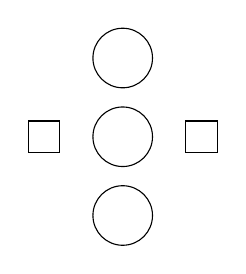
\begin{tikzpicture}
  \node[place]      (waiting 1)      at ( 0,2) {};
  \node[place]      (critical 1)     at ( 0,1) {};
  \node[place]      (semaphore)      at ( 0,0) {};
  \node[transition] (leave critical) at ( 1,1) {};
  \node[transition] (enter critical) at (-1,1) {};
\end{tikzpicture}
\end{dispExample*}


\switchcolumn[0]*%%%%%%%%%%%%
\subsection{Placing Nodes Using Relative Placement}
\switchcolumn
\subsection{使用相对定位放置节点}
\switchcolumn[0]*%%%%%%%%%%%%
Although Hagen still wishes to connect the nodes, he first wishes to address
another problem again: The placement of the nodes. Although he likes the |at|
syntax, in this particular case he would prefer placing the nodes ``relative to
each other''. So, Hagen would like to say that the |critical 1| node should be
below the |waiting 1| node, wherever the |waiting 1| node might be. There are
different ways of achieving this, but the nicest one in Hagen's case is the
|below| option:
\switchcolumn
虽然Hagen仍然希望连接节点,但他首先希望再次解决另一个问题:节点的放置。尽管他喜欢 |at| 语法,但在这种特殊情况下,他更愿意将节点“相对于彼此”放置。因此,Hagen希望指定 |critical 1| 节点应该在 |waiting 1| 节点的下方,无论 |waiting 1| 节点在哪里。有多种实现这一目标的方法,但在Hagen的情况下,最好的方法是使用 |below| 选项:
\switchcolumn[0]*%%%%%%%%%%%%
%\begin{codeexample}[preamble={\usetikzlibrary{positioning}}]
%\begin{tikzpicture}
%  \node[place]      (waiting)                            {};
%  \node[place]      (critical)       [below=of waiting]  {};
%  \node[place]      (semaphore)      [below=of critical] {};
%  \node[transition] (leave critical) [right=of critical] {};
%  \node[transition] (enter critical) [left=of critical]  {};
%\end{tikzpicture}
%\end{codeexample}
\begin{dispExample*}{sidebyside}
%preamble={\usetikzlibrary{positioning}}
\begin{tikzpicture}
  \node[place]      (waiting)                            {};
  \node[place]      (critical)       [below=of waiting]  {};
  \node[place]      (semaphore)      [below=of critical] {};
  \node[transition] (leave critical) [right=of critical] {};
  \node[transition] (enter critical) [left=of critical]  {};
\end{tikzpicture}
\end{dispExample*}
\switchcolumn
\begin{dispExample*}{sidebyside,lefthand ratio=0.7}
%preamble={\usetikzlibrary{positioning}}
\begin{tikzpicture}
  \node[place]      (waiting)                            {};
  \node[place]      (critical)       [below=of waiting]  {};
  \node[place]      (semaphore)      [below=of critical] {};
  \node[transition] (leave critical) [right=of critical] {};
  \node[transition] (enter critical) [left=of critical]  {};
\end{tikzpicture}
\end{dispExample*}
\switchcolumn[0]*%%%%%%%%%%%%
With the |positioning| library loaded, when an option like |below| is followed
by |of|, then the position of the node is shifted in such a manner that it is
placed at the distance |node distance| in the specified direction of the given
direction. The |node distance| is either the distance between the centers of
the nodes (when the |on grid| option is set to true) or the distance between
the borders (when the |on grid| option is set to false, which is the default).
\switchcolumn
加载 |positioning| 库后,当选项如 |below| 后面跟着 |of| 时,节点的位置会按照指定的方向在距离 |node distance| 处移动节点。|node distance| 是节点之间的距离(当将 |on grid| 选项设置为 true 时,为节点中心之间的距离),或者是边界之间的距离(当将 |on grid| 选项设置为 false,这是默认设置)。

\switchcolumn[0]*%%%%%%%%%%%%
Even though the above code has the same effect as the earlier code, Hagen can
pass it to his colleagues who will be able to just read and understand it,
perhaps without even having to see the picture.
\switchcolumn
尽管上面的代码与之前的代码具有相同的效果,但Hagen可以将其传递给他的同事,他们将能够只需阅读和理解它,甚至可能不必看到图片。
\switchcolumn[0]*%%%%%%%%%%%%
\switchcolumn[0]*%%%%%%%%%%%%
\subsection{Adding Labels Next to Nodes}
\switchcolumn
\subsection{在节点旁添加标签}
\switchcolumn[0]*%%%%%%%%%%%%
Before we have a look at how Hagen can connect the nodes, let us add the
capacity ``$s \le 3$'' to the bottom node. For this, two approaches are
possible:
\switchcolumn
在查看Hagen如何连接节点之前,让我们先在底部节点上添加容量“$s \le 3$”。有两种方法可以实现这一点:
\end{paracol}
%
\begin{enumerate}
\columnratio{0.55}
\begin{paracol}{2}
    \item Hagen can just add a new node above the |north| anchor of the
        |semaphore| node.
\switchcolumn	
\item  Hagen只需在 |semaphore| 节点的 |north| 锚点上方添加一个新节点。
\switchcolumn[0]*%%%%%%%%%%%%
\begin{dispExample*}{sidebyside,lefthand ratio=0.7}
%preamble={\usetikzlibrary{positioning}}
\begin{tikzpicture}
  \node[place]      (waiting)                            {};
  \node[place]      (critical)       [below=of waiting]  {};
  \node[place]      (semaphore)      [below=of critical] {};
  \node[transition] (leave critical) [right=of critical] {};
  \node[transition] (enter critical) [left=of critical]  {};

  \node [red,above] at (semaphore.north) {$s\le 3$};
\end{tikzpicture}
\end{dispExample*}
\switchcolumn
\begin{dispExample*}{sidebyside,lefthand ratio=0.7}
%preamble={\usetikzlibrary{positioning}}
\begin{tikzpicture}
  \node[place]      (waiting)                            {};
  \node[place]      (critical)       [below=of waiting]  {};
  \node[place]      (semaphore)      [below=of critical] {};
  \node[transition] (leave critical) [right=of critical] {};
  \node[transition] (enter critical) [left=of critical]  {};

  \node [red,above] at (semaphore.north) {$s\le 3$};
\end{tikzpicture}
\end{dispExample*}

        %
%\begin{codeexample}[preamble={\usetikzlibrary{positioning}}]
%\begin{tikzpicture}
%  \node[place]      (waiting)                            {};
%  \node[place]      (critical)       [below=of waiting]  {};
%  \node[place]      (semaphore)      [below=of critical] {};
%  \node[transition] (leave critical) [right=of critical] {};
%  \node[transition] (enter critical) [left=of critical]  {};

%  \node [red,above] at (semaphore.north) {$s\le 3$};
%\end{tikzpicture}
%\end{codeexample}
\switchcolumn[0]*%%%%%%%%%%%%
        This is a general approach that will ``always work''.
\switchcolumn
这是一种``始终有效''的通用方法。
\switchcolumn[0]*%%%%%%%%%%%%
    \item Hagen can use the special |label| option. This option is given to a
        |node| and it causes \emph{another} node to be added next to the node
        where the option is given. Here is the idea: When we construct the
        |semaphore| node, we wish to indicate that we want another node with
        the capacity above it. For this, we use the option
        |label=above:$s\le 3$|. This option is interpreted as follows: We want
        a node above the |semaphore| node and this node should read ``$s \le
        3$''. Instead of |above| we could also use things like |below left|
        before the colon or a number like |60|.
        %
\switchcolumn
\item Hagen可以使用特殊的 |label| 选项。这个选项适用于 |node|,它会导致在给出选项的节点旁边添加\emph{另一个}节点。这是思路:当我们构造 |semaphore| 节点时,我们希望指示我们想要在其上方有一个带有容量的节点。为此,我们使用选项 |label=above:$s\le 3$|。这个选项的解释如下:我们希望在 |semaphore| 节点上方有一个节点能够显示“$s \le 3$”。除了 |above|,我们还可以在冒号之前使用诸如 |below left| 这样的内容,或者使用数字如 |60|。
\switchcolumn[0]*%%%%%%%%%%%%
\begin{dispExample*}{sidebyside,lefthand ratio=0.7}
% preamble={\usetikzlibrary{positioning}}
\begin{tikzpicture}
\node[place]      (waiting)                            {};
\node[place]      (critical)       [below=of waiting]  {};
\node[place]      (semaphore)      [below=of critical,
                                    label=above:$s\le3$] {};
\node[transition] (leave critical) [right=of critical] {};
\node[transition] (enter critical) [left=of critical]  {};
\end{tikzpicture}
\end{dispExample*}
\switchcolumn
\begin{dispExample*}{sidebyside,lefthand ratio=0.7}
% preamble={\usetikzlibrary{positioning}}
\begin{tikzpicture}
  \node[place]      (waiting)                            {};
  \node[place]      (critical)       [below=of waiting]  {};
  \node[place]      (semaphore)      [below=of critical,
                                      label=above:$s\le3$] {};
  \node[transition] (leave critical) [right=of critical] {};
  \node[transition] (enter critical) [left=of critical]  {};
  \end{tikzpicture}
\end{dispExample*}

% \begin{codeexample}[preamble={\usetikzlibrary{positioning}}]
% \begin{tikzpicture}
%   \node[place]      (waiting)                            {};
%   \node[place]      (critical)       [below=of waiting]  {};
%   \node[place]      (semaphore)      [below=of critical,
%                                       label=above:$s\le3$] {};
%   \node[transition] (leave critical) [right=of critical] {};
%   \node[transition] (enter critical) [left=of critical]  {};
% \end{tikzpicture}
% \end{codeexample}
\switchcolumn[0]*%%%%%%%%%%%%
It is also possible to give multiple |label| options, this causes
multiple labels to be drawn.
\switchcolumn
同时可以给出多个 |label| 选项,这将导致绘制多个标签。
\switchcolumn[0]*%%%%%%%%%%%%
\begin{dispExample*}{sidebyside,lefthand ratio=0.7}
\tikz
  \node [circle,draw,label=60:$60^\circ$,label=below:$-90^\circ$] {my circle};
\end{dispExample*}
\switchcolumn
\begin{dispExample*}{sidebyside,lefthand ratio=0.9}
\tikz
  \node [circle,draw,label=60:$60^\circ$,label=below:$-90^\circ$] {my circle};
\end{dispExample*}

\switchcolumn[0]*%%%%%%%%%%%%
        Hagen is not fully satisfied with the |label| option since the label
        is not red. To achieve this, he has two options: First, he can
        redefine the |every label| style. Second, he can add options to the
        label's node. These options are given following the |label=|, so he
        would write |label=[red]above:$s\le3$|. However, this does not quite
        work since \TeX\ thinks that the |]| closes the whole option list of
        the |semaphore| node. So, Hagen has to add braces and writes
        |label={[red]above:$s\le3$}|. Since this looks a bit ugly, Hagen
        decides to redefine the |every label| style.
\switchcolumn
        Hagen对 |label| 选项并不完全满意,因为标签的颜色不是红色的。为了实现这一点,他有两个选项:首先,他可以重新定义 |every label| 样式。其次,他可以为标签的节点添加选项。这些选项在 |label=| 之后给出,因此他会写成 |label=[red]above:$s\le3$|。然而,这并不完全起作用,因为 \TeX\ 认为 |]| 关闭了整个 |semaphore| 节点的选项列表。因此,Hagen必须添加大括号,写成 |label={[red]above:$s\le3$}|。由于这看起来有点丑陋,Hagen决定重新定义 |every label| 样式。
\switchcolumn[0]*%%%%%%%%%%%%
\begin{dispExample*}{sidebyside,lefthand ratio=0.7}
%preamble={\usetikzlibrary{positioning}}
\begin{tikzpicture}[every label/.style={red}]
  \node[place]      (waiting)                            {};
  \node[place]      (critical)       [below=of waiting]  {};
  \node[place]      (semaphore)      [below=of critical,
                                      label=above:$s\le3$] {};
  \node[transition] (leave critical) [right=of critical] {};
  \node[transition] (enter critical) [left=of critical]  {};
\end{tikzpicture}
\end{dispExample*}
\switchcolumn
\begin{dispExample*}{sidebyside,lefthand ratio=0.7}
%preamble={\usetikzlibrary{positioning}}
\begin{tikzpicture}[every label/.style={red}]
  \node[place]      (waiting)                            {};
  \node[place]      (critical)       [below=of waiting]  {};
  \node[place]      (semaphore)      [below=of critical,
                                      label=above:$s\le3$] {};
  \node[transition] (leave critical) [right=of critical] {};
  \node[transition] (enter critical) [left=of critical]  {};
\end{tikzpicture}
\end{dispExample*}

% \begin{codeexample}[preamble={\usetikzlibrary{positioning}}]
% \begin{tikzpicture}[every label/.style={red}]
%   \node[place]      (waiting)                            {};
%   \node[place]      (critical)       [below=of waiting]  {};
%   \node[place]      (semaphore)      [below=of critical,
%                                       label=above:$s\le3$] {};
%   \node[transition] (leave critical) [right=of critical] {};
%   \node[transition] (enter critical) [left=of critical]  {};
% \end{tikzpicture}
% \end{codeexample}
\end{paracol}
\end{enumerate}


\columnratio{0.55}
\begin{paracol}{2}
\subsection{Connecting Nodes}
\switchcolumn
\subsection{连接节点}
\switchcolumn[0]*%%%%%%%%%%%%
It is now high time to connect the nodes. Let us start with something simple,
namely with the straight line from |enter critical| to |critical|. We want this
line to start at the right side of |enter critical| and to end at the left side
of |critical|. For this, we can use the \emph{anchors} of the nodes. Every node
defines a whole bunch of anchors that lie on its border or inside it. For
example, the |center| anchor is at the center of the node, the |west| anchor is
on the left of the node, and so on. To access the coordinate of a node, we use
a coordinate that contains the node's name followed by a dot, followed by the
anchor's name:
\switchcolumn
现在是时候连接节点了。让我们从简单的情况开始,即从 |enter critical| 到 |critical| 的直线。我们希望这条线从 |enter critical| 的右侧开始,结束在 |critical| 的左侧。为此,我们可以使用节点的\emph{锚点}。每个节点都定义了一组锚点,这些锚点位于其边界或内部。例如,|center| 锚点位于节点的中心,|west| 锚点位于节点的左侧,等等。要访问节点的坐标,我们使用包含节点名称、后跟一个点和锚点名称的坐标:
\switchcolumn[0]*%%%%%%%%%%%%
\begin{dispExample*}{sidebyside}
% preamble={\usetikzlibrary{positioning}}
\begin{tikzpicture}
\node[place]      (waiting)                            {};
\node[place]      (critical)       [below=of waiting]  {};
\node[place]      (semaphore)      [below=of critical] {};
\node[transition] (leave critical) [right=of critical] {};
\node[transition] (enter critical) [left=of critical]  {};
\draw [->] (enter critical.east) -- (critical.west);
\end{tikzpicture}
\end{dispExample*}
\switchcolumn
\begin{dispExample*}{sidebyside,lefthand ratio=0.7}
% preamble={\usetikzlibrary{positioning}}
\begin{tikzpicture}
\node[place]      (waiting)                            {};
\node[place]      (critical)       [below=of waiting]  {};
\node[place]      (semaphore)      [below=of critical] {};
\node[transition] (leave critical) [right=of critical] {};
\node[transition] (enter critical) [left=of critical]  {};
\draw [->] (enter critical.east) -- (critical.west);
\end{tikzpicture}
\end{dispExample*}

% \begin{codeexample}[preamble={\usetikzlibrary{positioning}}]
% \begin{tikzpicture}
%   \node[place]      (waiting)                            {};
%   \node[place]      (critical)       [below=of waiting]  {};
%   \node[place]      (semaphore)      [below=of critical] {};
%   \node[transition] (leave critical) [right=of critical] {};
%   \node[transition] (enter critical) [left=of critical]  {};
%   \draw [->] (enter critical.east) -- (critical.west);
% \end{tikzpicture}
% \end{codeexample}

\switchcolumn[0]*%%%%%%%%%%%%
Next, let us tackle the curve from |waiting| to |enter critical|. This can be
specified using curves and controls:
\switchcolumn
接下来,让我们来处理从 |waiting| 到 |enter critical| 的曲线。这可以使用曲线和控制点来指定:
\switchcolumn[0]*%%%%%%%%%%%%
\begin{dispExample*}{sidebyside}
% \usetikzlibrary{positioning}
\begin{tikzpicture}
  \node[place]      (waiting)                            {};
  \node[place]      (critical)       [below=of waiting]  {};
  \node[place]      (semaphore)      [below=of critical] {};
  \node[transition] (leave critical) [right=of critical] {};
  \node[transition] (enter critical) [left=of critical]  {};
  \draw [->] (enter critical.east) -- (critical.west);
  \draw [->] (waiting.west) .. controls +(left:5mm) and +(up:5mm)
                            .. (enter critical.north);
\end{tikzpicture}
\end{dispExample*}
\switchcolumn
\begin{dispExample*}{sidebyside,lefthand ratio=0.7}
% \usetikzlibrary{positioning}
\begin{tikzpicture}
  \node[place]      (waiting)                            {};
  \node[place]      (critical)       [below=of waiting]  {};
  \node[place]      (semaphore)      [below=of critical] {};
  \node[transition] (leave critical) [right=of critical] {};
  \node[transition] (enter critical) [left=of critical]  {};
  \draw [->] (enter critical.east) -- (critical.west);
  \draw [->] (waiting.west) .. controls +(left:5mm) and +(up:5mm)
                            .. (enter critical.north);
\end{tikzpicture}
\end{dispExample*}
 
% \begin{codeexample}[preamble={\usetikzlibrary{positioning}}]
% \begin{tikzpicture}
%   \node[place]      (waiting)                            {};
%   \node[place]      (critical)       [below=of waiting]  {};
%   \node[place]      (semaphore)      [below=of critical] {};
%   \node[transition] (leave critical) [right=of critical] {};
%   \node[transition] (enter critical) [left=of critical]  {};
%   \draw [->] (enter critical.east) -- (critical.west);
%   \draw [->] (waiting.west) .. controls +(left:5mm) and +(up:5mm)
%                             .. (enter critical.north);
% \end{tikzpicture}
% \end{codeexample}
\switchcolumn[0]*%%%%%%%%%%%%
Hagen sees how he can now add all his edges, but the whole process seems a but
awkward and not very flexible. Again, the code seems to obscure the structure
of the graphic rather than showing it.
\switchcolumn
Hagen看到他现在可以添加所有的边,但整个过程似乎有些别扭,而且不太灵活。再一次,代码似乎掩盖了图形的结构,而不是展示出来。

\switchcolumn[0]*%%%%%%%%%%%%
So, let us start improving the code for the edges. First, Hagen can leave out
the anchors:
\switchcolumn
因此,让我们开始改进边的代码。首先,Hagen可以省略锚点:

\switchcolumn[0]*%%%%%%%%%%%%
%
\begin{codeexample}[preamble={\usetikzlibrary{positioning}}]
\begin{tikzpicture}
  \node[place]      (waiting)                            {};
  \node[place]      (critical)       [below=of waiting]  {};
  \node[place]      (semaphore)      [below=of critical] {};
  \node[transition] (leave critical) [right=of critical] {};
  \node[transition] (enter critical) [left=of critical]  {};
  \draw [->] (enter critical) -- (critical);
  \draw [->] (waiting) .. controls +(left:8mm) and +(up:8mm)
                       .. (enter critical);
\end{tikzpicture}
\end{codeexample}

Hagen is a bit surprised that this works. After all, how did \tikzname\ know
that the line from |enter critical| to |critical| should actually start on the
borders? Whenever \tikzname\ encounters a whole node name as a ``coordinate'',
it tries to ``be smart'' about the anchor that it should choose for this node.
Depending on what happens next, \tikzname\ will choose an anchor that lies on
the border of the node on a line to the next coordinate or control point. The
exact rules are a bit complex, but the chosen point will usually be correct --
and when it is not, Hagen can still specify the desired anchor by hand.
\switchcolumn

\switchcolumn[0]*%%%%%%%%%%%%
Hagen would now like to simplify the curve operation somehow. It turns out that
this can be accomplished using a special path operation: the |to| operation.
This operation takes many options (you can even define new ones yourself). One
pair of options is useful for Hagen: The pair |in| and |out|. These options
take angles at which a curve should leave or reach the start or target
coordinates. Without these options, a straight line is drawn:
%
\begin{codeexample}[preamble={\usetikzlibrary{positioning}}]
\begin{tikzpicture}
  \node[place]      (waiting)                            {};
  \node[place]      (critical)       [below=of waiting]  {};
  \node[place]      (semaphore)      [below=of critical] {};
  \node[transition] (leave critical) [right=of critical] {};
  \node[transition] (enter critical) [left=of critical]  {};
  \draw [->] (enter critical) to                 (critical);
  \draw [->] (waiting)        to [out=180,in=90] (enter critical);
\end{tikzpicture}
\end{codeexample}

There is another option for the |to| operation, that is even better suited to
Hagen's problem: The |bend right| option. This option also takes an angle, but
this angle only specifies the angle by which the curve is bent to the right:
\switchcolumn

\switchcolumn[0]*%%%%%%%%%%%%
%
\begin{codeexample}[preamble={\usetikzlibrary{positioning}}]
\begin{tikzpicture}
  \node[place]      (waiting)                            {};
  \node[place]      (critical)       [below=of waiting]  {};
  \node[place]      (semaphore)      [below=of critical] {};
  \node[transition] (leave critical) [right=of critical] {};
  \node[transition] (enter critical) [left=of critical]  {};
  \draw [->] (enter critical) to                 (critical);
  \draw [->] (waiting)        to [bend right=45] (enter critical);
  \draw [->] (enter critical) to [bend right=45] (semaphore);
\end{tikzpicture}
\end{codeexample}

It is now time for Hagen to learn about yet another way of specifying edges:
Using the |edge| path operation. This operation is very similar to the |to|
operation, but there is one important difference: Like a node the edge
generated by the |edge| operation is not part of the main path, but is added
only later. This may not seem very important, but it has some nice
consequences. For example, every edge can have its own arrow tips and its own
color and so on and, still, all the edges can be given on the same path. This
allows Hagen to write the following:
%
\begin{codeexample}[preamble={\usetikzlibrary{positioning}}]
\begin{tikzpicture}
  \node[place]      (waiting)                            {};
  \node[place]      (critical)       [below=of waiting]  {};
  \node[place]      (semaphore)      [below=of critical] {};
  \node[transition] (leave critical) [right=of critical] {};
  \node[transition] (enter critical) [left=of critical]  {}
    edge [->]               (critical)
    edge [<-,bend left=45]  (waiting)
    edge [->,bend right=45] (semaphore);
\end{tikzpicture}
\end{codeexample}

Each |edge| caused a new path to be constructed, consisting of a |to| between
the node |enter critical| and the node following the |edge| command.
\switchcolumn

\switchcolumn[0]*%%%%%%%%%%%%
The finishing touch is to introduce two styles |pre| and |post| and to use the
|bend angle=45| option to set the bend angle once and for all:
\switchcolumn

\switchcolumn[0]*%%%%%%%%%%%%
%
\begin{codeexample}[preamble={\usetikzlibrary{arrows.meta,positioning}}]
% Styles place and transition as before
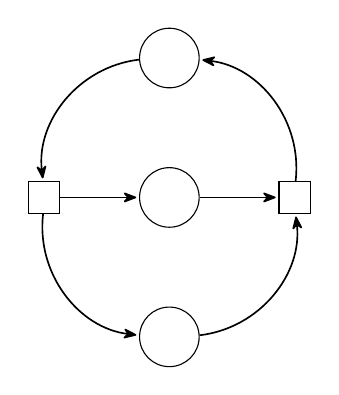
\begin{tikzpicture}
  [bend angle=45,
   pre/.style={<-,shorten <=1pt,>={Stealth[round]},semithick},
   post/.style={->,shorten >=1pt,>={Stealth[round]},semithick}]

  \node[place]      (waiting)                            {};
  \node[place]      (critical)       [below=of waiting]  {};
  \node[place]      (semaphore)      [below=of critical] {};

  \node[transition] (leave critical) [right=of critical] {}
    edge [pre]             (critical)
    edge [post,bend right] (waiting)
    edge [pre, bend left]  (semaphore);
  \node[transition] (enter critical) [left=of critical]  {}
    edge [post]            (critical)
    edge [pre, bend left]  (waiting)
    edge [post,bend right] (semaphore);
\end{tikzpicture}
\end{codeexample}


\subsection{Adding Labels Next to Lines}
\switchcolumn

\switchcolumn[0]*%%%%%%%%%%%%
The next thing that Hagen needs to add is the ``$2$'' at the arcs. For this
Hagen can use \tikzname's automatic node placement: By adding the option
|auto|, \tikzname\ will position nodes on curves and lines in such a way that
they are not on the curve but next to it. Adding |swap| will mirror the label
with respect to the line. Here is a general example:
%
% TODOsp: codeexamples: styles not needed here
\begin{dispExample*}{sidebyside}
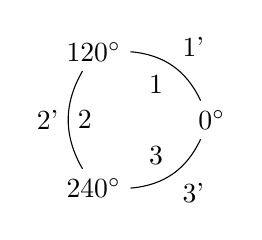
\begin{tikzpicture}[auto,bend right]
  \node (a) at (0:1) {$0^\circ$};
  \node (b) at (120:1) {$120^\circ$};
  \node (c) at (240:1) {$240^\circ$};

  \draw (a) to node {1} node [swap] {1'} (b)
        (b) to node {2} node [swap] {2'} (c)
        (c) to node {3} node [swap] {3'} (a);
\end{tikzpicture}
\end{dispExample*}
\switchcolumn
\begin{dispExample*}{sidebyside}
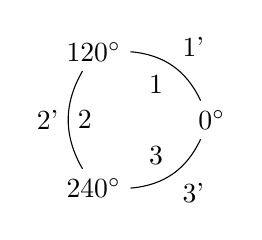
\begin{tikzpicture}[auto,bend right]
  \node (a) at (0:1) {$0^\circ$};
  \node (b) at (120:1) {$120^\circ$};
  \node (c) at (240:1) {$240^\circ$};

  \draw (a) to node {1} node [swap] {1'} (b)
        (b) to node {2} node [swap] {2'} (c)
        (c) to node {3} node [swap] {3'} (a);
\end{tikzpicture}
\end{dispExample*}


What is happening here? The nodes are given somehow inside the |to| operation!
When this is done, the node is placed on the middle of the curve or line
created by the |to| operation. The |auto| option then causes the node to be
moved in such a way that it does not lie on the curve, but next to it. In the
example we provide even two nodes on each |to| operation.
\switchcolumn

\switchcolumn[0]*%%%%%%%%%%%%
For Hagen that |auto| option is not really necessary since the two ``2'' labels
could also easily be placed ``by hand''. However, in a complicated plot with
numerous edges automatic placement can be a blessing.
\switchcolumn

\switchcolumn[0]*%%%%%%%%%%%%
%
\begin{codeexample}[
    preamble={\usetikzlibrary{arrows.meta,positioning}},
    pre={\tikzset{
    pre/.style={<-,shorten <=1pt,>={Stealth[round]},semithick},
    post/.style={->,shorten >=1pt,>={Stealth[round]},semithick},
}},
]
% Styles as before
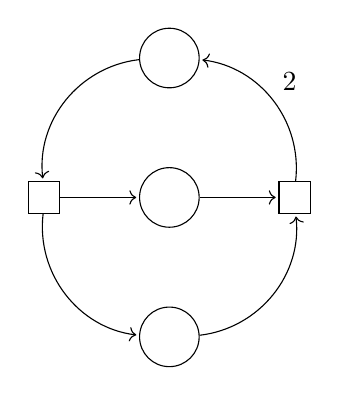
\begin{tikzpicture}[bend angle=45]
  \node[place]      (waiting)                            {};
  \node[place]      (critical)       [below=of waiting]  {};
  \node[place]      (semaphore)      [below=of critical] {};

  \node[transition] (leave critical) [right=of critical] {}
    edge [pre]                                 (critical)
    edge [post,bend right] node[auto,swap] {2} (waiting)
    edge [pre, bend left]                      (semaphore);
  \node[transition] (enter critical) [left=of critical]  {}
    edge [post]                                (critical)
    edge [pre, bend left]                      (waiting)
    edge [post,bend right]                     (semaphore);
\end{tikzpicture}
\end{codeexample}
% TODOsp: codeexamples: styles and `positioning` are needed up to here


\subsection{Adding the Snaked Line and Multi-Line Text}
\switchcolumn

\switchcolumn[0]*%%%%%%%%%%%%
With the node mechanism Hagen can now easily create the two Petri nets. What he
is unsure of is how he can create the snaked line between the nets.
\switchcolumn

\switchcolumn[0]*%%%%%%%%%%%%
For this he can use a \emph{decoration}. To draw the snaked line, Hagen only
needs to set the two options |decoration=snake| and |decorate| on the path.
This causes all lines of the path to be replaced by snakes. It is also possible
to use snakes only in certain parts of a path, but Hagen will not need this.
%
\begin{codeexample}[preamble={\usetikzlibrary{decorations.pathmorphing}}]
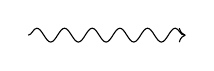
\begin{tikzpicture}
  \draw [->,decorate,decoration=snake] (0,0) -- (2,0);
\end{tikzpicture}
\end{codeexample}

Well, that does not look quite right, yet. The problem is that the snake
happens to end exactly at the position where the arrow begins. Fortunately,
there is an option that helps here. Also, the snake should be a bit smaller,
which can be influenced by even more options.
\switchcolumn

\switchcolumn[0]*%%%%%%%%%%%%
%
\begin{codeexample}[preamble={\usetikzlibrary{decorations.pathmorphing}}]
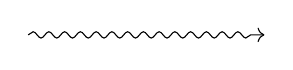
\begin{tikzpicture}
  \draw [->,decorate,
     decoration={snake,amplitude=.4mm,segment length=2mm,post length=1mm}]
    (0,0) -- (3,0);
\end{tikzpicture}
\end{codeexample}

Now Hagen needs to add the text above the snake. This text is a bit challenging
since it is a multi-line text. Hagen has two options for this: First, he can
specify an |align=center| and then use the |\\| command to enforce the line
breaks at the desired positions.
%
\begin{codeexample}[preamble={\usetikzlibrary{decorations.pathmorphing}}]
\begin{tikzpicture}
  \draw [->,decorate,
      decoration={snake,amplitude=.4mm,segment length=2mm,post length=1mm}]
    (0,0) -- (3,0)
    node [above,align=center,midway]
    {
      replacement of\\
      the \textcolor{red}{capacity}\\
      by \textcolor{red}{two places}
    };
\end{tikzpicture}
\end{codeexample}

Instead of specifying the line breaks ``by hand'', Hagen can also specify a
width for the text and let \TeX\ perform the line breaking for him:
\switchcolumn

\switchcolumn[0]*%%%%%%%%%%%%
%
\begin{codeexample}[preamble={\usetikzlibrary{decorations.pathmorphing}}]
\begin{tikzpicture}
  \draw [->,decorate,
      decoration={snake,amplitude=.4mm,segment length=2mm,post length=1mm}]
    (0,0) -- (3,0)
    node [above,text width=3cm,align=center,midway]
    {
      replacement of the \textcolor{red}{capacity} by
      \textcolor{red}{two places}
    };
\end{tikzpicture}
\end{codeexample}


\subsection{Using Layers: The Background Rectangles}
\switchcolumn

\switchcolumn[0]*%%%%%%%%%%%%
Hagen still needs to add the background rectangles. These are a bit tricky:
Hagen would like to draw the rectangles \emph{after} the Petri nets are
finished. The reason is that only then can he conveniently refer to the
coordinates that make up the corners of the rectangle. If Hagen draws the
rectangle first, then he needs to know the exact size of the Petri net -- which
he does not.
\switchcolumn

\switchcolumn[0]*%%%%%%%%%%%%
The solution is to use \emph{layers}. When the |backgrounds| library is loaded,
Hagen can put parts of his picture inside a scope with the
|on background layer| option. Then this part of the picture becomes part of the
layer that is given as an argument to this environment. When the
|{tikzpicture}| environment ends, the layers are put on top of each other,
starting with the background layer. This causes everything drawn on the
background layer to be behind the main text.
\switchcolumn

\switchcolumn[0]*%%%%%%%%%%%%
The next tricky question is, how big should the rectangle be? Naturally, Hagen
can compute the size ``by hand'' or using some clever observations concerning
the $x$- and $y$-coordinates of the nodes, but it would be nicer to just have
\tikzname\ compute a rectangle into which all the nodes ``fit''. For this, the
|fit| library can be used. It defines the |fit| options, which, when given to a
node, causes the node to be resized and shifted such that it exactly covers all
the nodes and coordinates given as parameters to the |fit| option.
\switchcolumn

\switchcolumn[0]*%%%%%%%%%%%%
%
% TODOsp: codeexamples: redo/add styles starting from here
\begin{codeexample}[
    preamble={\usetikzlibrary{arrows.meta,backgrounds,fit,positioning}},
    pre={\tikzset{
    pre/.style={<-,shorten <=1pt,>={Stealth[round]},semithick},
    post/.style={->,shorten >=1pt,>={Stealth[round]},semithick},
}},
]
% Styles as before
\begin{tikzpicture}[bend angle=45]
  \node[place]      (waiting)                            {};
  \node[place]      (critical)       [below=of waiting]  {};
  \node[place]      (semaphore)      [below=of critical] {};

  \node[transition] (leave critical) [right=of critical] {}
    edge [pre]                                 (critical)
    edge [post,bend right] node[auto,swap] {2} (waiting)
    edge [pre, bend left]                      (semaphore);
  \node[transition] (enter critical) [left=of critical]  {}
    edge [post]                                (critical)
    edge [pre, bend left]                      (waiting)
    edge [post,bend right]                     (semaphore);

  \begin{scope}[on background layer]
    \node [fill=black!30,fit=(waiting) (critical) (semaphore)
             (leave critical) (enter critical)] {};
  \end{scope}
\end{tikzpicture}
\end{codeexample}


\subsection{The Complete Code}
\switchcolumn

\switchcolumn[0]*%%%%%%%%%%%%
Hagen has now finally put everything together. Only then does he learn that
there is already a library for drawing Petri nets! It turns out that this
library mainly provides the same definitions as Hagen did. For example, it
defines a |place| style in a similar way as Hagen did. Adjusting the code so
that it uses the library shortens Hagen code a bit, as shown in the following.
\switchcolumn

\switchcolumn[0]*%%%%%%%%%%%%
First, Hagen needs less style definitions, but he still needs to specify the
colors of places and transitions.
\switchcolumn

\switchcolumn[0]*%%%%%%%%%%%%
%
\begin{codeexample}[code only]
\begin{tikzpicture}
  [node distance=1.3cm,on grid,>={Stealth[round]},bend angle=45,auto,
   every place/.style=     {minimum size=6mm,thick,draw=blue!75,fill=blue!20},
   every transition/.style={thick,draw=black!75,fill=black!20},
   red place/.style=       {place,draw=red!75,fill=red!20},
   every label/.style=     {red}]
\end{codeexample}

Now comes the code for the nets:
\switchcolumn

\switchcolumn[0]*%%%%%%%%%%%%
%
\ifpgfmanualexternalize\tikzexternaldisable\fi
\begin{codeexample}[
    preamble={\usetikzlibrary{arrows.meta,petri,positioning}},
    pre={\tikzset{
    every place/.style={minimum size=6mm,thick,draw=blue!75,fill=blue!20},
    every transition/.style={thick,draw=black!75,fill=black!20},
    every label/.style={red},
    every picture/.style={on grid,node distance=1.3cm,>={Stealth[round]},bend angle=45,auto},
}%
\begin{tikzpicture}},
    post={\end{tikzpicture}},
]
   \node [place,tokens=1] (w1)                                    {};
   \node [place]          (c1) [below=of w1]                      {};
   \node [place]          (s)  [below=of c1,label=above:$s\le 3$] {};
   \node [place]          (c2) [below=of s]                       {};
   \node [place,tokens=1] (w2) [below=of c2]                      {};

   \node [transition] (e1) [left=of c1] {}
     edge [pre,bend left]                  (w1)
     edge [post,bend right]                (s)
     edge [post]                           (c1);
   \node [transition] (e2) [left=of c2] {}
     edge [pre,bend right]                 (w2)
     edge [post,bend left]                 (s)
     edge [post]                           (c2);
   \node [transition] (l1) [right=of c1] {}
     edge [pre]                            (c1)
     edge [pre,bend left]                  (s)
     edge [post,bend right] node[swap] {2} (w1);
   \node [transition] (l2) [right=of c2] {}
     edge [pre]                            (c2)
     edge [pre,bend right]                 (s)
     edge [post,bend left]  node {2}       (w2);
\end{codeexample}

\ifpgfmanualexternalize\tikzexternaldisable\fi
\begin{codeexample}[
    preamble={\usetikzlibrary{arrows.meta,petri,positioning}},
    pre={\tikzset{
    every place/.style={minimum size=6mm,thick,draw=blue!75,fill=blue!20},
    every transition/.style={thick,draw=black!75,fill=black!20},
    red place/.style=  {place,draw=red!75,fill=red!20},
    every label/.style={red},
    every picture/.style={on grid,node distance=1.3cm,>={Stealth[round]},bend angle=45,auto},
}%
\begin{tikzpicture}},
    post={\end{tikzpicture}},
]
  \begin{scope}[xshift=6cm]
    \node [place,tokens=1]     (w1')                            {};
    \node [place]              (c1') [below=of w1']             {};
    \node [red place]          (s1') [below=of c1',xshift=-5mm]
            [label=left:$s$]                                    {};
    \node [red place,tokens=3] (s2') [below=of c1',xshift=5mm]
            [label=right:$\bar s$]                              {};
    \node [place]              (c2') [below=of s1',xshift=5mm]  {};
    \node [place,tokens=1]     (w2') [below=of c2']             {};

    \node [transition] (e1') [left=of c1'] {}
      edge [pre,bend left]                  (w1')
      edge [post]                           (s1')
      edge [pre]                            (s2')
      edge [post]                           (c1');
    \node [transition] (e2') [left=of c2'] {}
      edge [pre,bend right]                 (w2')
      edge [post]                           (s1')
      edge [pre]                            (s2')
      edge [post]                           (c2');
    \node [transition] (l1') [right=of c1'] {}
      edge [pre]                            (c1')
      edge [pre]                            (s1')
      edge [post]                           (s2')
      edge [post,bend right] node[swap] {2} (w1');
    \node [transition] (l2') [right=of c2'] {}
      edge [pre]                            (c2')
      edge [pre]                            (s1')
      edge [post]                           (s2')
      edge [post,bend left]  node {2}       (w2');
  \end{scope}
\end{codeexample}

The code for the background and the snake is the following:
\switchcolumn

\switchcolumn[0]*%%%%%%%%%%%%
%
\begin{codeexample}[code only]
  \begin{scope}[on background layer]
    \node (r1) [fill=black!10,rounded corners,fit=(w1)(w2)(e1)(e2)(l1)(l2)] {};
    \node (r2) [fill=black!10,rounded corners,fit=(w1')(w2')(e1')(e2')(l1')(l2')] {};
  \end{scope}

  \draw [shorten >=1mm,->,thick,decorate,
         decoration={snake,amplitude=.4mm,segment length=2mm,
                     pre=moveto,pre length=1mm,post length=2mm}]
    (r1) -- (r2) node [above=1mm,midway,text width=3cm,align=center]
      {replacement of the \textcolor{red}{capacity} by \textcolor{red}{two places}};
\end{tikzpicture}
\end{codeexample}

% -----------------------------------------------------------------------------
% TODOsp: codeexamples: This is needed because -- unlike I thought --
%         `setup code is remembered also outside this file. Thus the changed
%         style of `place` and `transition` are "remembered" in
%         <pgfmanual-en-library-petri.tex>
\begin{codeexample}[setup code,hidden]
% from <tikzlibrarypetri.code.tex>
\tikzset{
    place/.style={circle,draw,inner sep=0pt,minimum size=5ex,every place},
    transition/.style={rectangle,draw,inner sep=0pt,minimum size=4mm,every transition},
}
\end{codeexample}
% -----------------------------------------------------------------------------

\end{paracol}